% ============================================
% SECTION 1: Introduction
% ============================================
\section{Introdução}

\begin{frame}{Contexto}
\begin{itemize}
    \item Documentos são fundamentais na sociedade corporativa
    \begin{itemize}
        \item Contratos, relacionamentos empregatícios, empréstimos, identidades
    \end{itemize}
    \item Digitalização crescente, mas muitas organizações ainda recebem documentos físicos
    \item Pipeline de entendimento de documentos necessário:
    \begin{enumerate}
        \item Verificação da forma (tipo correto de documento)
        \item Extração de informações para decisões de negócio
    \end{enumerate}
\end{itemize}
\begin{center}
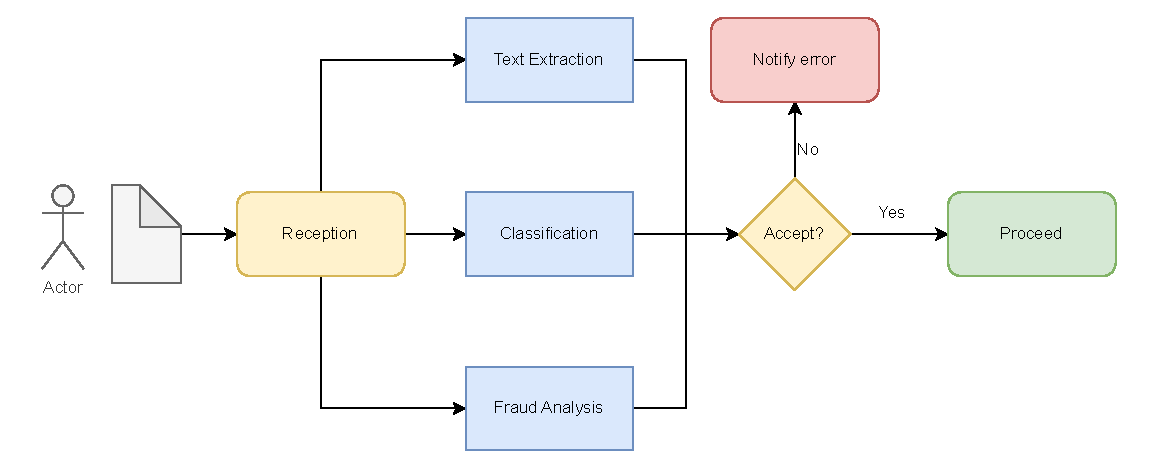
\includegraphics[width=0.7\textwidth]{images/diagrama-compliance.drawio.pdf}
\end{center}
\end{frame}

\begin{frame}{Document Image Classification (DIC)}
\begin{columns}
\column{0.5\textwidth}
\textbf{Classificação Tradicional:}
\begin{itemize}
    \item Categorização em classes predefinidas
    \item Informação textual nem sempre disponível
    \item Entrada: fotos ou scans de documentos
    \item Uso de OCR quando necessário
\end{itemize}

\textbf{Desempenho Atual:}
\begin{itemize}
    \item Bakkali et al. (2021): 97.70\% de acurácia no RVL-CDIP
\end{itemize}

\column{0.5\textwidth}
\textbf{O Problema:}
\begin{itemize}
    \item Novos layouts de documentos
    \item Classes completamente novas
    \item Necessidade de retreinamento
    \item Semanas/meses de engenharia de dados e treinamento
\end{itemize}

\textbf{Solução:}
\begin{itemize}
    \item Técnicas de Zero-Shot Learning (ZSL)
    \item Generalização para classes não vistas
\end{itemize}
\end{columns}
\end{frame}

\begin{frame}{Problema de Pesquisa}
\begin{block}{Desafios em ZSL para DIC}
\begin{enumerate}
    \item \textbf{Falta de dataset especializado}
    \begin{itemize}
        \item Datasets existentes não têm splits disjuntos entre treino e teste
        \item Informação insuficiente para treinar modelos ZSL eficientes
    \end{itemize}
    
    \item \textbf{Ausência de metodologia estado-da-arte}
    \begin{itemize}
        \item Trabalhos usam metodologias próprias e incomparáveis
        \item Uso extensivo de LLMs pré-treinados (custo elevado)
    \end{itemize}
    
    \item \textbf{Dificuldades com datasets existentes}
    \begin{itemize}
        \item RVL-CDIP não é adequado para ZSL (F1 score de apenas 69.9\%)
        \item Classes definidas por propósito, não por estrutura visual
    \end{itemize}
\end{enumerate}
\end{block}
\end{frame}

\begin{frame}{Contribuições deste Trabalho}
\begin{enumerate}
    \item \textbf{Novo dataset de imagens de documentos}
    \begin{itemize}
        \item Especificamente projetado para classificação ZSL
        \item Focado em padrões visuais/estruturais
    \end{itemize}
    
    \item \textbf{Abordagem de Visual Document Matching (VDM)}
    \begin{itemize}
        \item Baseada em similaridade de imagens
        \item Técnicas de aprendizado métrico
        \item Generalização para layouts não vistos
    \end{itemize}
    
    \item \textbf{Avaliação sistemática}
    \begin{itemize}
        \item Benchmarking de múltiplos backbones estabelecidos
        \item Comparação com Large Language Models
        \item Referências valiosas para pesquisas futuras
    \end{itemize}
\end{enumerate}
\end{frame}
